\documentclass[a4paper,11pt,pdftex,halfparskip,cleardoubleempty,bibtotoc,liststotoc]{scrbook}

\raggedbottom

% \usepackage{fancyhdr}

\usepackage[utf8]{inputenc}
\usepackage{wrapfig}
\usepackage[pdftex]{graphicx}
\usepackage{eso-pic}
\usepackage{array}
\usepackage{tabularx}
\usepackage{xcolor}
\usepackage{float}
\usepackage{listings}
\usepackage[toc,page]{appendix}

\setlength{\tabcolsep}{20pt}
\renewcommand{\arraystretch}{4}

\graphicspath{{img/}}
\newcommand*{\xchapter}{\stepcounter{chapter}\setcounter{section}{0}\addchap}
%\renewcommand*{\thesection}{\arabic{section}}

%\chapterstyle{hangnum}

\usepackage{xcolor}

\definecolor{codegreen}{rgb}{0,0.6,0}
\definecolor{codegray}{rgb}{0.5,0.5,0.5}
\definecolor{codepurple}{rgb}{0.58,0,0.82}
\definecolor{backcolour}{rgb}{0.95,0.95,0.92}

\lstdefinestyle{mystyle}{
    backgroundcolor=\color{backcolour},   
    commentstyle=\color{codegreen},
    keywordstyle=\color{magenta},
    numberstyle=\tiny\color{codegray},
    stringstyle=\color{codepurple},
    basicstyle=\ttfamily\footnotesize,
    breakatwhitespace=false,         
    breaklines=true,                 
    captionpos=b,                    
    keepspaces=true,                 
    numbers=left,                    
    numbersep=5pt,                  
    showspaces=false,                
    showstringspaces=false,
    showtabs=false,                  
    tabsize=2
}

\lstset{style=mystyle}

% define medatata
\def\MTitle{High-Level Modeling and Low-Level Adaption of Serverless Function Choreographies}
\def\MAuthor{Benjamin Walch}
\def\MKeywords{Serverless \sep Function Choreography Language}
\def\MOrg{Universit{\"a}t Innsbruck}
\def\MDate{\today}
\def\MInstitution{Department of Computer Science}
\def\MSupervisor{Dr. Shashko Ristov}
\def\MGroup{Distributed and Parallel Systems}

%
% \pagestyle{fancy}
% \fancyhf{}
% \fancyhead[L]{\leftmark}
% \fancyhead[R]{\thepage}
% \fancyfoot[R]{B. Walch}
% \fancyfoot[L]{Fastlane}

\begin{document}

\frontmatter
\pagestyle{empty}

\begin{titlepage}
\rule{0mm}{1mm}

\begin{multicols}{2}[\columnsep2em] 
	
\includegraphics[width=6cm]{uibk-logo}
	\columnbreak
	\begin{flushright}
		\Large{\textsf{\MOrg}}
	\end{flushright}
\end{multicols}

\begin{flushright}
	{\large \MInstitution\\}
	{\large \MGroup}
\end{flushright}

\vspace*{1.5cm}

\begin{center}
	{\LARGE\bf \MTitle}
	\vskip 2.25cm
	\Large \textbf{Bachelor Thesis}
	\vskip 2.25cm
	{\Large \MAuthor}
	\vskip 1.5cm
	{\large Supervisor: \MSupervisor}   
	\vfill
	{\large Innsbruck, \MDate}
\end{center}
%\AddToShipoutPicture{
%	\put(-55,55){
%		\parbox[b]{\paperwidth}{
%			\hfill 
\includegraphics[scale=0.35]{uibk-watermark}
%		}
%	}
%}
\end{titlepage} 

\ClearShipoutPicture

\cleardoublepage

\section*{Eidesstaatliche Erklärung}

Ich erkläre hiermit an Eides statt durch meine eigenhändige Unterschrift, dass ich die vorliegende Arbeit selbständig verfasst und keine anderen als die angegebenen Quellen und Hilfsmittel verwendet habe. Alle Stellen, die wörtlich oder inhaltlich den angegebenen Quellen entnommen wurden, sind als solche kenntlich gemacht.

Ich erkläre mich mit der Archivierung der vorliegenden Bachelorarbeit einverstanden.

\vspace{1.8cm}

\parbox{6cm}{
	\hrule
	\strut \centering\footnotesize Datum
} \hfill
\parbox{6cm}{
	\hrule
	\strut \centering\footnotesize Unterschrift
}

\cleardoublepage

\pagenumbering{arabic}
\pagestyle{plain}

\chapter*{Abstract}

% to be written at the end!
% some results ..

The Distributed and Parallel Systems group developed the \emph{Abstract Function Choreography Language} (AFCL). It is a specification for describing serverless workflows. Furthermore, a Java API, to describe serverless application workflows programmatically, was developed.
The product which results in using that API is a workflow being described in AFCL in a text based file.
Until now, the workflow being described in the text file has to be created manually (by editing the file directly), or a programmer has to write Java code which utilizes the API to generate the file.
\par
The aim of this bachelor project is to develop a visual workflow editor, which makes modeling of workflows possible at a high level of abstraction. The tool should not only be able to load, display and save workflows, but also optimize workflows for multiple FaaS provider(s) in case of quotas and limits, and also in case of performance.

\cleardoublepage

\tableofcontents

\newpage

\label{sec:introduction}
\chapter{Introduction}

% - Why is the work important?
% - provider specific implementations
% - need tool to create easily 


% In the FaaS world, there exist many providers who offer serverless execution of code (functions) in the cloud. Each of them has its own specifications and definitions on how functions are deployed and executed, and how workflows are created and executed.
"Run code, not Servers" is a recent term in the cloud computing world.
With the rise of serverless technologies during the last years, \emph{Function-as-a-Service} (FaaS) became more and more popular. This cloud computing concept offers new advantages for software development: very high flexibility, nearly unlimited scalability and pay-per-use pricing. Global Players like Amazon, Google, IBM and Microsoft jumped on the train and provide their infrastructure to developers, with the ability to deploy and execute their code in the cloud. 

Moving from \emph{Infrastucture-as-a-service} (IaaS) over \emph{Platform-as-a-service} (Paas) to Faas, developers can completely focus on the program they need to run and not worry at all about the machine it is on or the resources it requires \cite{articles-going-serverless-savage}.
An entire program can be defined by a workflow, which in turn consists of functions. Workflows, though, can be executed using serverless technology in the cloud.

Many providers offer a tool to create a workflow and execute it (Amazon Step Functions, IBM Cloud Functions, Microsoft Azure Functions, Google Cloud Functions, ...). Most of them also offer the option to export the composed workflow to a text file.
But each provider has its own definitions on how a workflow is expressed, as well as different pricing models, limits and quotas. Additionally, different providers also support different programming languages. That being said, a workflow from one system is not compatible with another, what means, the user is bound to a specific provider, if he wants to reuse or change a workflow later.

The distributed and parallel systems group developed a specification to describe serverless function choreographies generically. This specification is called \emph{Abstract Function Choreography Language} (AFCL) and was developed to eliminate incompatibility of workflows between different providers. 

\section{Objective}

Castro et al. mentions that "One of the major challenges slowing the adoption of serverless is the lack of tools and frameworks" \cite{articles-rise-of-serverless-castro}. 

Therefore, this thesis has the goal to implement a new tool providing a graphical user interface for modeling workflows and export them in AFCL. In addition, loading and visualizing of existing workflows should be supported.
The tool should also be able to optimize composed workflows.

It is assumed that concrete implementations of the functions are already developed and deployed to a FaaS provider.
  
\section{Requirements}

\begin{itemize}
	\item design for the overall application [coreUI]
	\item clean and intuitive UI [bootstrap]
	\item ability to add components/menu points easily [modularity]
	\item good user experience [SPA]
	\item frameworks: open source, large community (future-safe)
	\item cross-browser [?]
	\item performance [?]
\end{itemize}
\begin{itemize}
	\item open-source
	\item good documentation
	\item actively maintained
	\item large and active community (future-proof)
	\item stars on github / downloads on npmtrends
	\item performance
	\item pre-knowledge of the developer / learning curve
\end{itemize}

%Describing the implementation in the next section 2

%This thesis is structured in three parts. At the beginning there is a short introduction to Faas, followed by explanations and additional information about AFCL.
%After that 

\chapter{Background}

This chapter contains important details on the terms and technologies used in this thesis and helps the reader to better understand the further topics.\\
First of all, the serverless concept, in particular \emph{Function-as-a-Service}, Workflows and Functions are explained, before giving a short overview about AFCL. The tools and technologies used for the development are also presented to readers who are not yet familiar with them.

\section{Serverless Computing}

Serverless computing is widely known as an event-driven cloud execution model. In this model, the client provides the code and the cloud provider manages the life-cycle of the execution environment of that code.
The idea is based on reducing the life span of the program to execute functionality in response to an event. Hence, the program's processes are born when an event is triggered and are killed after the event is processed \cite{inproceedings-serverless-beyond-the-cloud-kanso}.

Castro et al. define serverless computing as follows: "Serverless comuting is a platform that hides server usage from developers and runs code on-demand automatically scaled and billed only for the time the code is running" \cite{articles-rise-of-serverless-castro}.

The term ‘serverless’ can be misleading though, as there are still servers providing these backend services, but all of the server space and infrastructure concerns are handled by the vendor. Serverless means that the developers can do their work without having to worry about servers at all \cite{online-what-is-serverless-cloudflare}.



\section{Workflows and Functions}


\section{AFCL}

\section{Development Tools and Technologies}
\subsection{npm}

The node package manager\footnote{https://www.npmjs.org} is the world's largest software registry, where open-source software packages of developers and companies are shared all over the world. Over the last years, npm became a de-facto standard for package management in JavaScript development.

\subsection{webpack}

webpack is a module bundler, its main purpose is to bundle JavaScript code for the usage in a browser.\footnote{https://webpack.js.org} In particular, multiple modules (often hundreds of) with dependencies [to each other] are processed and bundled into a few files. To be able to process other types of files than JavaScript or JSON, webpack offers the opportunity to configure a \textbf{loader}. In this application, the following loaders are configured:
\begin{itemize}
\item babel-loader, to transform ECMAScript and React JSX to browser-compatible JavaScript
\item sass-loader, to transform SASS to CSS
\item css-loader, to transform CSS to CommonJS
\item file-loader, to handle static resources like images and fonts
\end{itemize}

\subsection{ECMAScript}

The scripting language specification ECMAScript (ES) was created to standardize JavaScript. With the release of ES6 (also known as ECMAScript 2015), features like class declarations, module imports and arrow function expressions became possible. After ES6, every year a new edition of the ECMAScript standard was finalized and released, offering new features. Worth mentioning here is the rest/spread operator released with ES9, which occurs a lot in the source code of this thesis.\\
% spread operator is a lot in use in source code
Since current browsers only have partial support of ECMAScript, a 'transcompiler' (or transpiler) is needed to transform the ECMAScript source code to JavaScript, which common browsers are capable of interpreting.
This compiling process is done with Babel\footnote{https://babeljs.io}, which is configured to not only compile ECMAScript, but also JSX to JavaScript.

\subsection{SASS}

CSS, in its pure form, reaches its limits when one thinks about using variables, functions or nested rules. SASS\footnote{https://sass-lang.com} is a stylesheet language, which is - similiar to ES - compiled to CSS and offers the mentioned and even more features.
A lot of CSS Frameworks also provide their source code in SASS, often served with a large variable set which makes it easy to customize it. The transpiler used in this thesis to transform SASS to CSS is node-sass\footnote{https://github.com/sass/node-sass}.


\chapter{Implementation}

% what the system does, what if offers

The Implementation of a Graphical User Interface as well as the optimization of workflows were the main goals of this bachelor thesis.

%A prototyping phase was the kickoff for the development: Different frameworks and libraries have been researched, tested and selected. The result of this phase was a working prototype as proof-of-concept.
% In order to achieve the goals, i did the following ...

\section{Architecture}

% show interfaces between modules
% Input output in each
% communication
% (to subsystems: FE constists of this ..., BE constists of this - goals of both BE and FE)
% more grained visualization

Operating mostly decoupled from one another, the application  consists of two sub systems - a Java backend and a web-based frontend. Those communicate and share JSON encoded objects between each other through an API the backend provides and the frontend consumes. The backend is responsible for converting and optimizing workflows at low-level as well as persisting of function data. The conversion of workflows is needed because the frontend encodes the visual representation of a workflow in XML, which is given as input to the backend. The conversion process is done by utilizing the AFCL API. 

The frontend displays and controls the application's user interface. It is responsible for visualizing the data and provide the canvas where the user can compose a workflow.

\begin{figure}[H]
  \centering
  \vspace{0.8cm}
  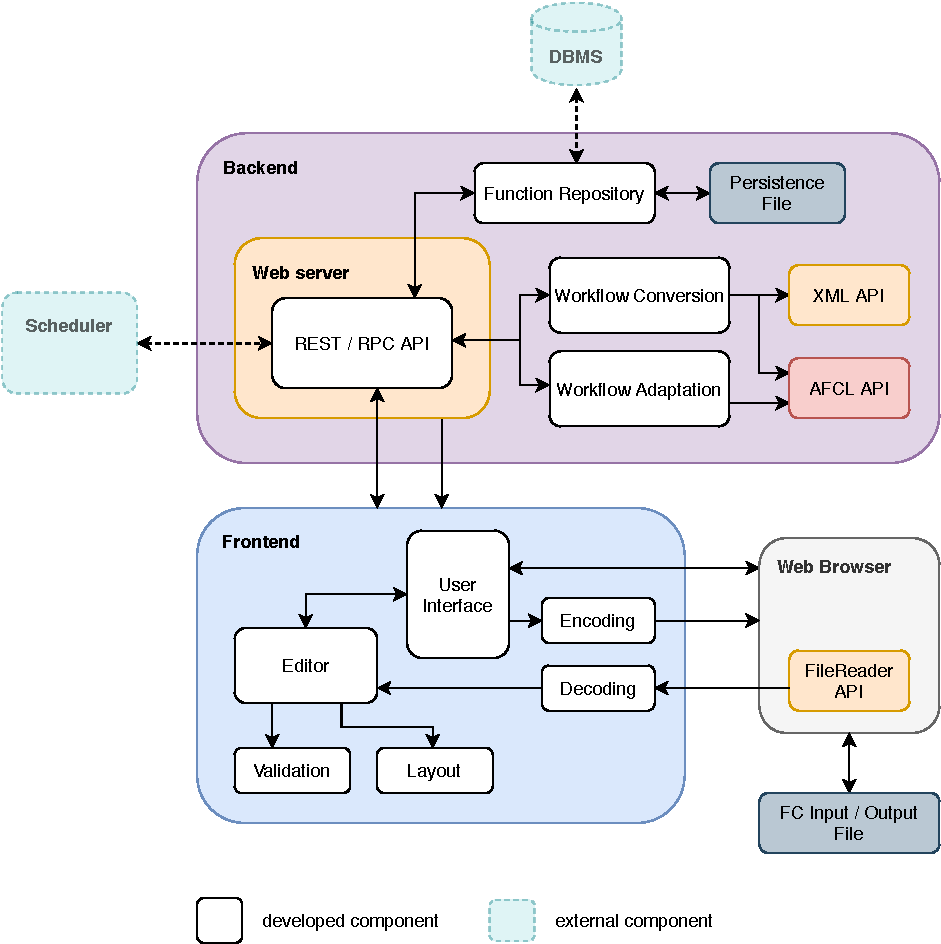
\includegraphics[scale=0.8]{architecture}
  \caption{application architecture}
\end{figure}

\section{Frontend}
Since a web based frontend which runs in the user's web browser, is a hard requirement, the core technologies are limited to HTML, CSS and JavaScript.


% add definitions here (EcmaScript JavaScript SASS ...)

% \subsection{Development Workflow}
% SYSTEM DESIGN
\subsection{Setup}

The setup of the frontend application is a selection of tools and technologies for modern and complex web development.
The base forms the node package manager (npm) which is used to manage and resolve the dependencies. Additionally, npm's CLI is used as tool to execute development and build tasks.

Under the hood, JavaScript and several JavaScript Frameworks are in action to control the application consisting of several UI components. To give the application its look and feel, CSS and some CSS Frameworks are in use.

Webpack does much of heavy-lifting, by bundling all sources with the assets into single files, and execute additional build steps by utilizing so-called 'loaders'.
Babel is used as such a webpack loader, for compiling the ECMAScript and React JSX source code to browser-compatible JavaScript.
The same applies for the CSS extension SASS, which is also integrated as a webpack loader, and is used to make the process of styling the user interface more efficient.

% Subsystem design
\begin{figure}[htbp]
  \centering
  \vspace{0.8cm}
  \includegraphics[width=\textwidth]{frontend-setup}
  \caption{frontend development toolchain}
\end{figure}
%%% TECHNOLOGIES / TOOLS %%%

\subsection{Data model}

All AFCL Java model classes have been ported to ECMAScript, to have all classes and properties available in the frontend, similiar like they are in the backend. Although plain JavaScript objects would also do the job, this adds a kind of type-safety to the ECMAScript sources and improves readability of the code. Also, the data exchange with the backend and the encoding of the graph benefit from this approach, since the XML node names map to constructor names.

\subsection{Graph drawing}

A workflow can be visualized as a directed graph.
The graph library used in this thesis to visualize a workflow is the JavaScript portion of mxGraph\footnote{https://jgraph.github.io/mxgraph/}. It is actively maintained and developed (during the development of the frontend, three bugfix releases and one minor release have been made public) and has an outstanding documentation. Additionally, it has a lot of demos and example code which show a lot of use cases and extensive features. Furthermore it integrates easily with React.

Basically, vertices and edges are represented by an \texttt{mxCell} model, which stores information about the cell's position, dimension, geometry and style.
Additionally, a user object can be attached to a \texttt{mxCell}. User objects give the graph its context, they store the business logic associated with the visual part. In this application, the cell's user objects are instances of AFCL objects.

Thus, the graph visualizes the execution sequence of the workflow.

% table vertices and user objects

\subsubsection{Validation}

\subsubsection{Encoding}

\subsubsection{Alternatives}

One of the more difficult tasks was to choose a proper library for graph drawing. Since the graph drawing and visualization is one of the most important features of the frontend, a careful choice has to be made. Of course there exist multiple excellent JavaScript graph drawing libraries. 

Below is a list of tested and researched JavaScript graph libraries with additional information why they were insufficient for the project.
\begin{itemize}
	\item \textbf{jsPlumb} is a library of great quality and looks like it would fulfill all  requirements for graph drawing and user interaction out of the box. It has a very good documentation, and a lot of examples. Furthermore its animations and drag and drop handling are outstandingly good. Unfortunately this software is not open source and a license costs a few thousand dollars.
	\item The same goes for \textbf{Rappid} (formerly known as JointJS) and \textbf{GoJS}, which is even more expensive.
	\item \textbf{diagram-js} is one of the newer diagram libraries. It seems to be a good candidate to draw BPMN\footnote{http://www.bpmn.org} graphs. The lack of an appropriate documentation - even after 4 years of existence (there exists an open issue on github\footnote{https://github.com/bpmn-io/diagram-js/issues/78} for this) - is still an issue.
	\item \textbf{Cytoscape.js} is older than mxGraph but the development and the community is not less active. This library has a very good documentation and a lot of demos are provided. But it offers fewer examples and "out-of-the-box" features for modeling flowcharts than mxGraph does.
	\item \textbf{vis.js} is a star on npmtrends.\footnote{https://www.npmtrends.com/vis}  It has very smooth animations when manipulating the graph. There exists only one example of graph manipulation on its documentation, it is mainly used for visualization only.
	\item \textbf{Sigma js} is a tiny library with a small documentation. It clearly focuses on displaying and visualizing graphs, not on modeling them. This part would have to be developed manually. Furthermore, the last activity on this project on github was 2 years ago.
\end{itemize}

\subsection{Web Interface}

The layout of the web interface is based on coreUI\footnote{https://coreui.io}, an admin panel template, built on top of the web toolkit Bootstrap\footnote{https://getbootstrap.com}. A clean and nested structure of components, which is typical for a React app, guarantees modularity and forms the whole frontend application. One of the benefits when using React is that the data model displayed to the user maps most of the time nicely to UI components. Basically, the components of the application respect the single responsibility principle\footnote{https://en.wikipedia.org/wiki/Single\_responsibility\_principle}. The main component has four sub-components - where each of them consists again of multiple sub-components - representing the core features of the app.

\subsubsection{Dashboard}

The dashboard is the entry point where the user lands after accessing the app. The purpose of this component is to give the user a quick overview of the application, provide short informational texts and links to the specific modules. 

\begin{figure}[H]
  \centering
  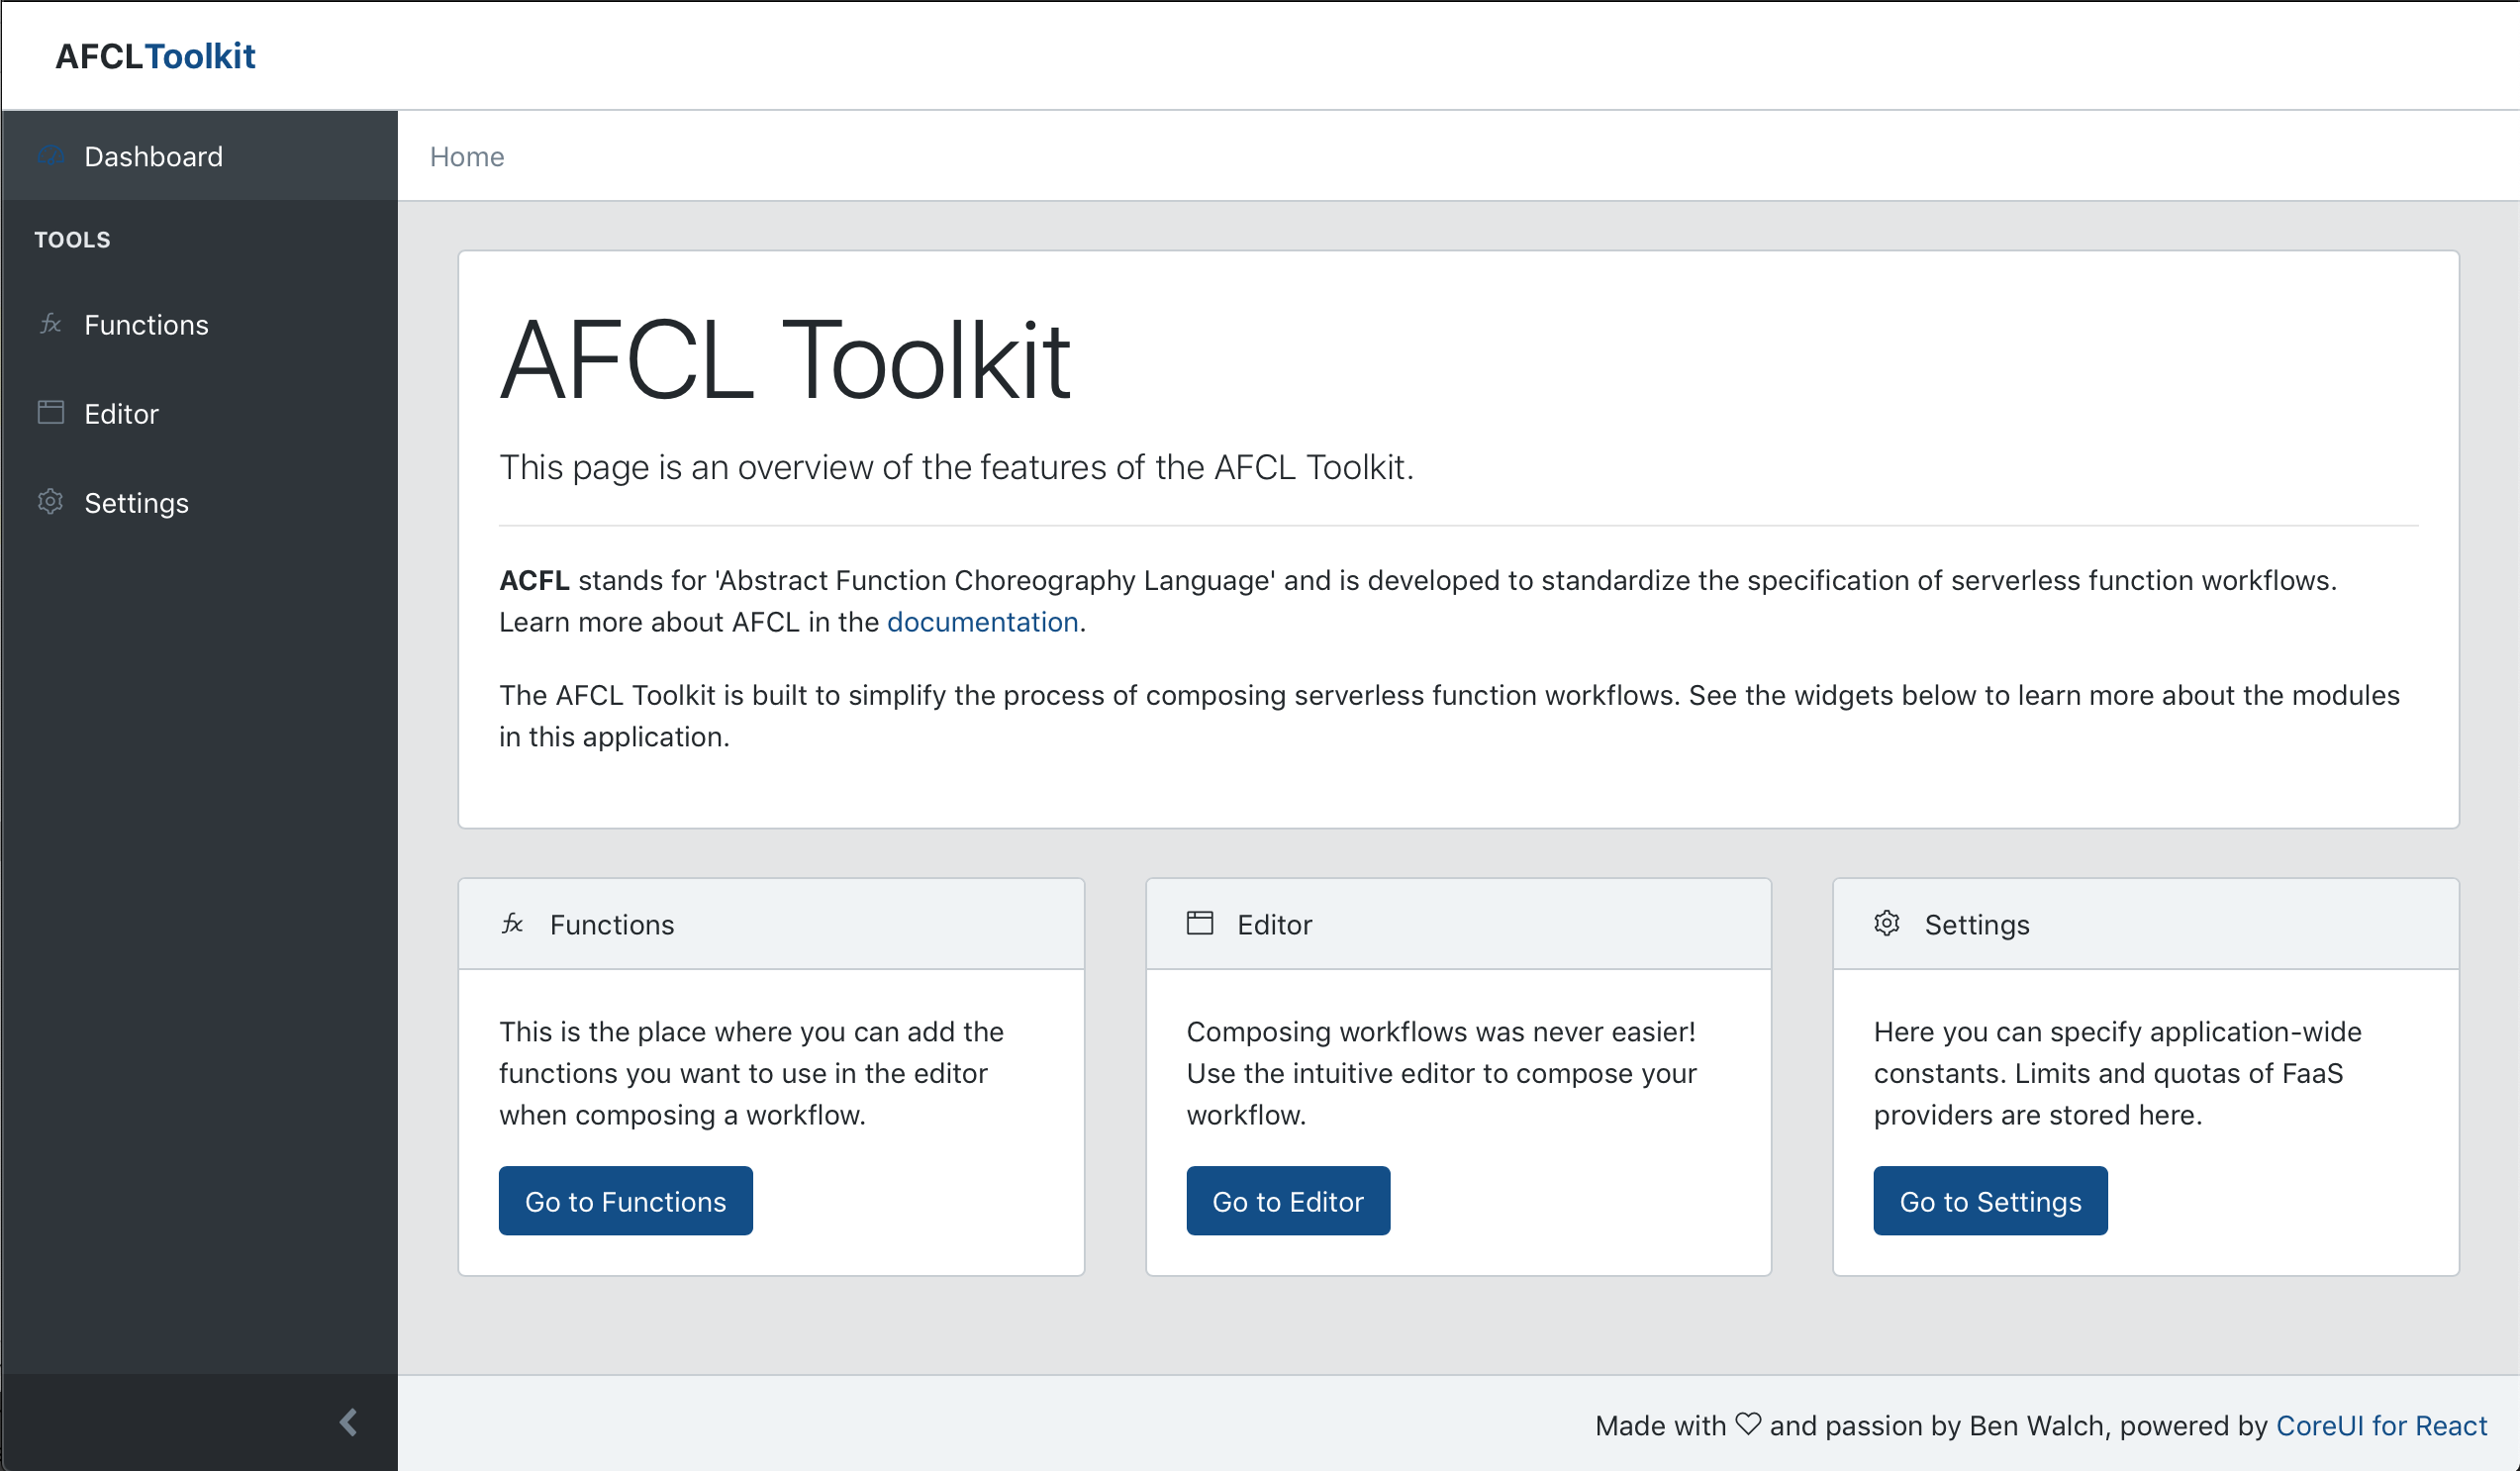
\includegraphics[width=\textwidth]{dashboard}
  \caption{the dashboard}
\end{figure}

\subsubsection{Functions}

A function repository is needed to know about available functions when composing a workflow. An item in the function repository holds the following data: name, type and provider. For In the implementation of this thesis, this data is persisted to an internal file.\footnote{see \ref{Backend-Persistence} for detailed information on how data is persisted}

\begin{figure}[H]
  \centering
  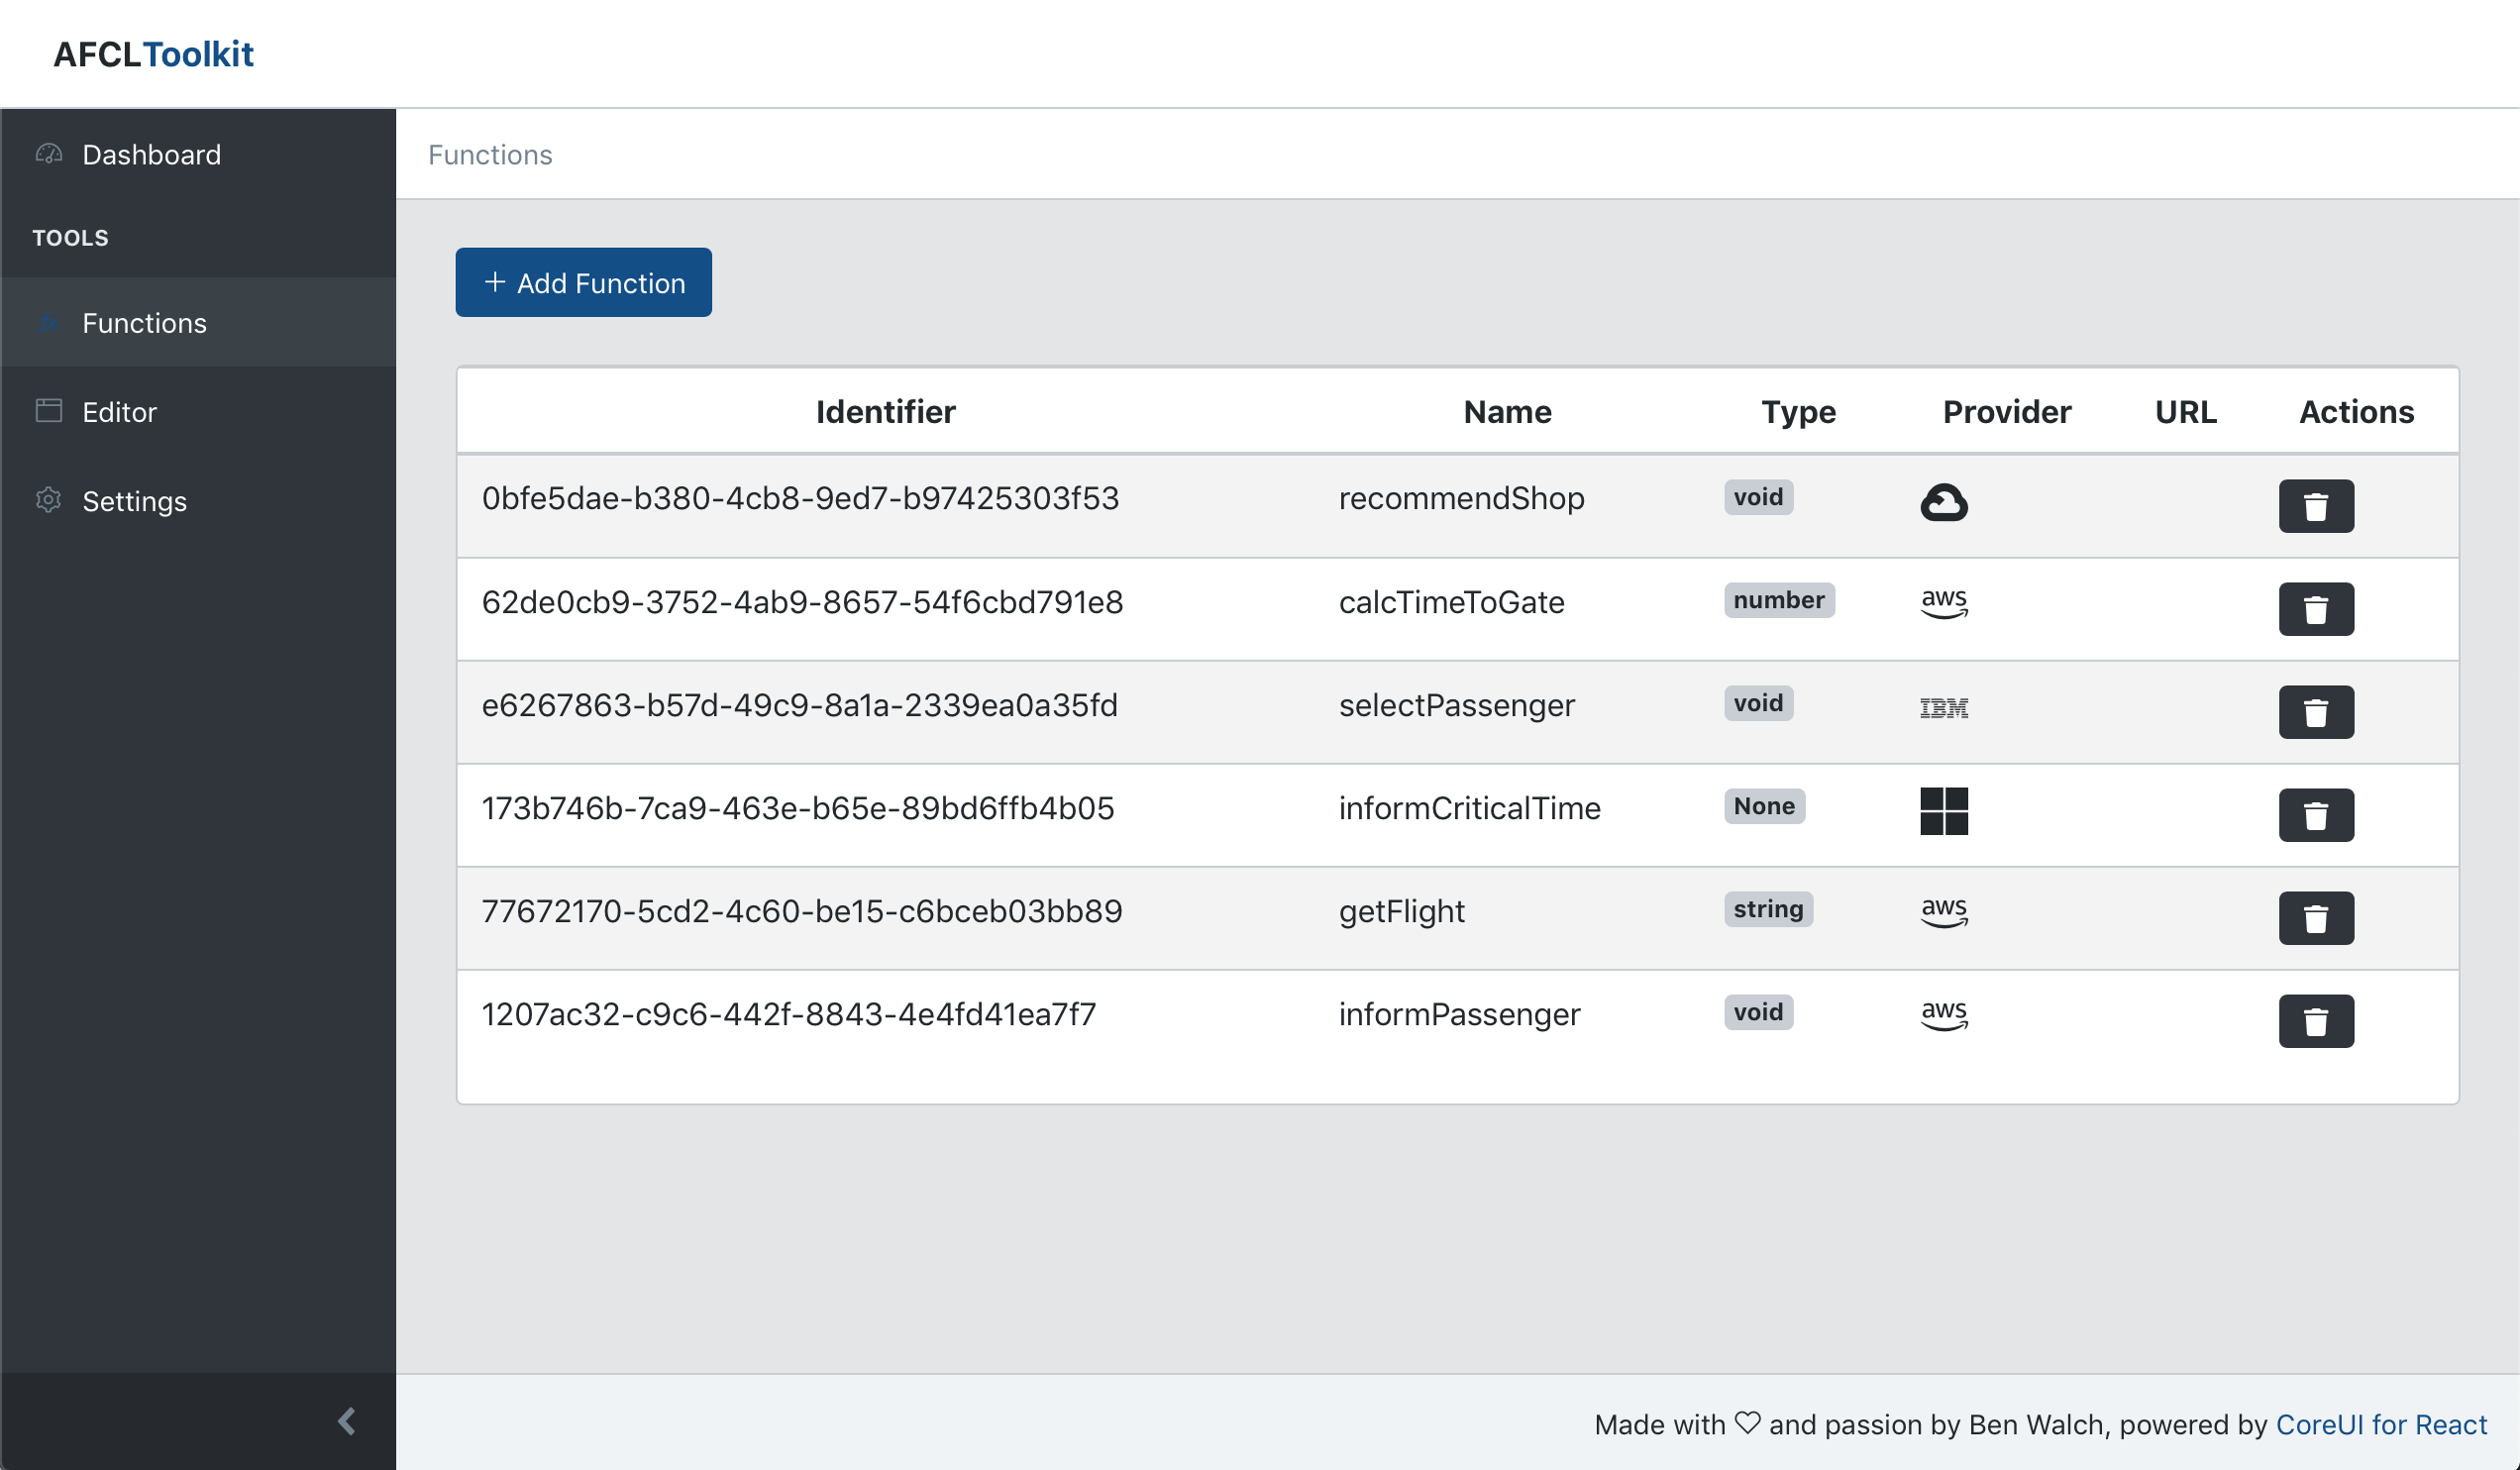
\includegraphics[width=\textwidth]{functions}
  \caption{the function repository}
\end{figure}

\subsubsection{Editor}
\par
The interface of the component responsible for composing workflows is divided into two parts. On the left side is the editor, consisting of a toolbar and a drawing area, on the right side is the property view. In the editor, the user can choose a function from the toolbar to place it in the drawing area below.  For the sake of clarity, each function has a defined shape and style. In the drawing area, these shapes (functions) can then be connected to each other by drag and drop. This leads to a directed graph, which represent the execution flow. The possible connection points (ports) of a shape will be displayed when hovering over it. These ports are input and output for most of the functions. When hovering a port, the port name appears in the tooltip.
\par
When selecting a shape in the canvas, the property view changes. It displays each specific property of the selected function, with the ability to change, add or remove properties.

\begin{figure}[H]
  \centering
  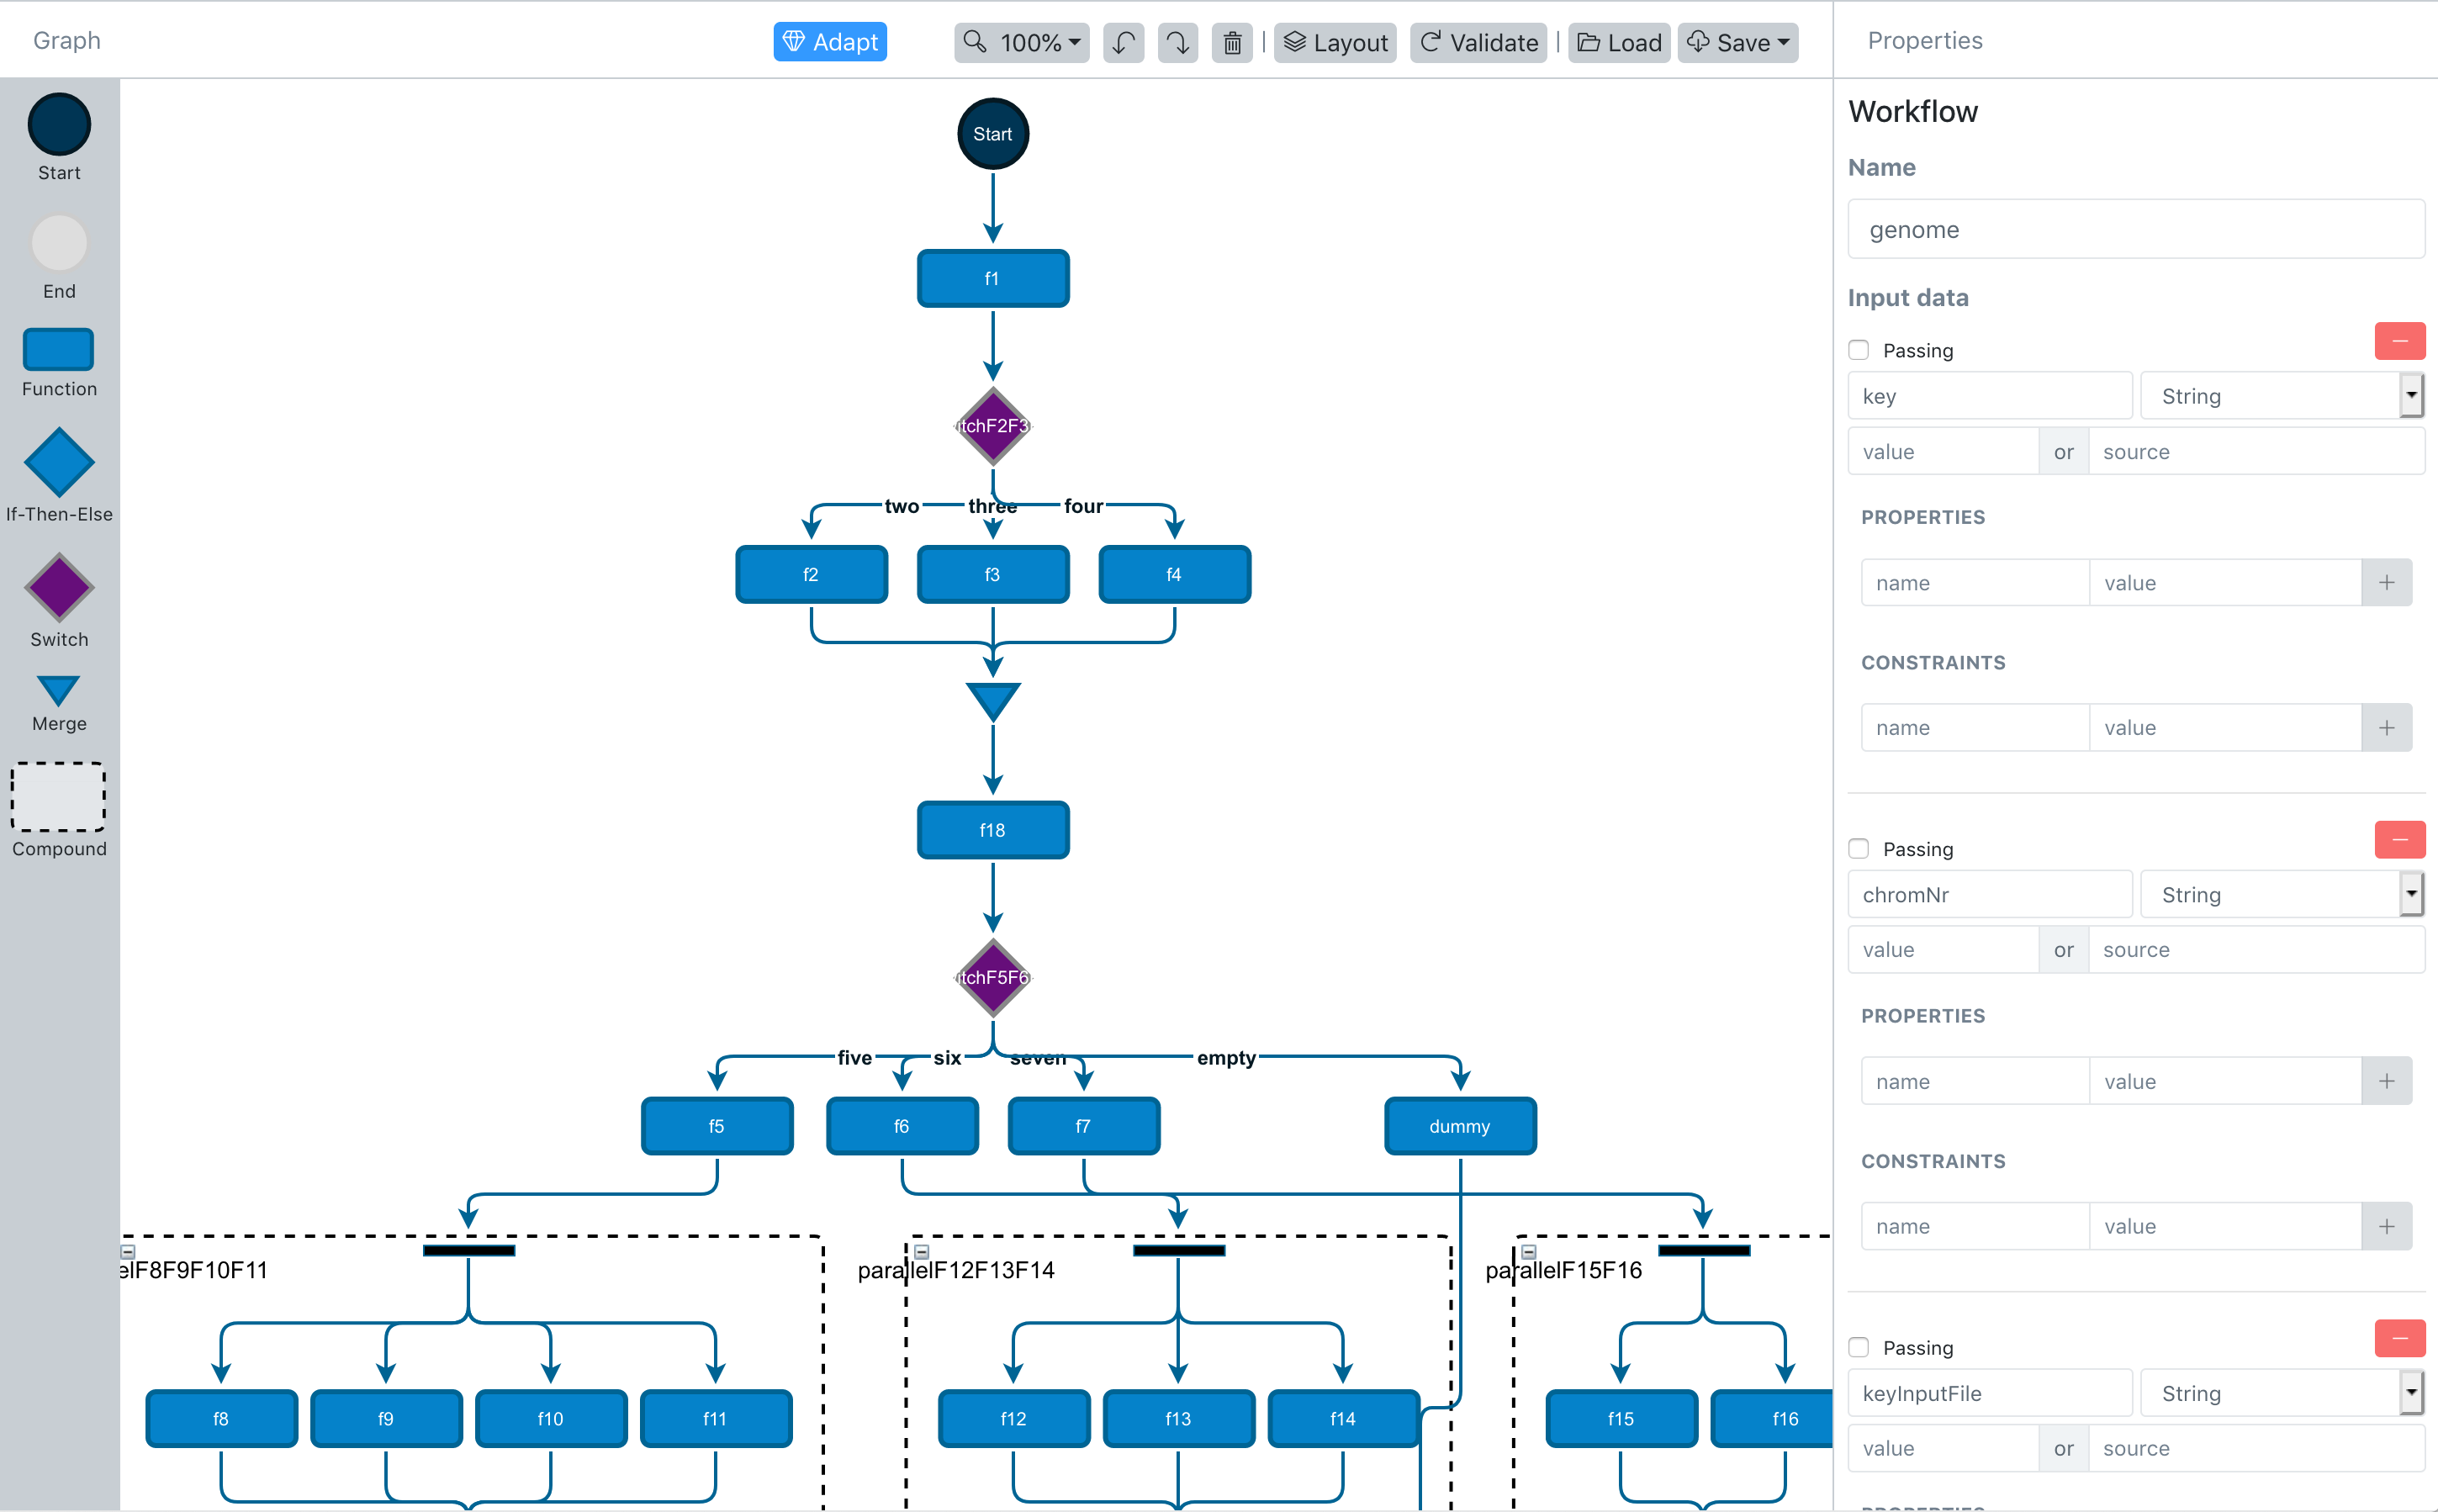
\includegraphics[width=\textwidth]{editor}
  \caption{the editor}
\end{figure}

\subsubsection{Settings}

\section{Backend}
\subsection{Setup}
 Maven, Servlets

\subsection{Api}

RESTful (Functions) and RPC-Style (Workflows)
% https://www.smashingmagazine.com/2016/09/understanding-rest-and-rpc-for-http-apis/

\subsection{Decoding}
 XML is good because built-in XPath support in Java.
\subsection{Persistence}
\label{Backend-Persistence}

Composed workflows are saved to the user's file system by offering a download. The user can then choose the target location.
The storing of function data, on the other hand, is abstracted from the user and persisting of the data is handled internally.
An interface\footnote{https://docs.oracle.com/javase/specs/jls/se7/html/jls-9.html} for the repository implementation was created on the backend side to be capable of supporting any data source. The repository which implements the interface in this thesis, stores the serialized data into a file. This could be easily replaced with any other implementation, for example an implementation which stores the data in a DBMS.

\begin{lstlisting}[language=Java, caption=Repository Interface]
public interface Repository<T> {

    public Collection<T> findAll();

    public T findOne(String id);

    public void add(T obj);

    public void remove(T obj);

    public void remove(String id);

    public void update(T obj);
}
\end{lstlisting}

\subsection{Optimization}

% interface so that someone can update the yaml file based on 
% decision

\section{Continuous Delivery}

\chapter{Evaluation}

% manually vs modeling -> what is the benefit
% compare manually vs modeling (time)
% for a workflow of size X benefit is 30%
% more quality typo-safe

\chapter{Conclusion}


% causes to print all bibliography
\nocite{*}

\bibliographystyle{ieeetr}
\bibliography{thesis.bib}

\end{document} 
